%% AMS-LaTeX Created by Wolfram Mathematica 9.0 : www.wolfram.com

\documentclass{article}
\usepackage{amsmath, amssymb, graphics, setspace}
\usepackage{graphicx}
\usepackage{xcolor}
\usepackage{hyperref}
\usepackage{tikz}
\usepackage[utf8]{inputenc}
\usepackage{spverbatim}
\usepackage{geometry}
 \geometry{
 a4paper,
 left=15mm,
 right=10mm,
 top=20mm,
 bottom=20mm,
 }

\DeclareMathSizes{10}{10}{10}{10}

\newcommand{\mathsym}[1]{{}}
\newcommand{\unicode}[1]{{}}

\newcounter{mathematicapage}
\begin{document}


\section{Ondas de sonido}
Una perturbación de pequeña amplitud en un fluido va a crear zonas de compresión y rarefacción que alternan en el tiempo y espacio en la dirección de propagación(el movimiento oscilatorio de las particulas se propaga como una onda y son ondas logitudinales:  las particulas se mueven en la misma dirección que la dirección de propagación)

\paragraph{Condiciones iniciales}
Consideramos un fluido ideal con las variables velocidad, densidad y presión(dependen de x y t) en el estado de equilibrio 
$v_{00} = 0, \rho_0 , p_0$ ($p_0, \rho_0$ constantes en el caso homogeneo, variando lentamente en espacio y/o tiempo en el caso inhomogeneo)
 y hacemos unos cambios en estas variables añadiendo unas perturbaciones:
$ v, \rho\prime, p\prime $ 
que  son muy pequeñas de forma que se pueden omitir los términos de segundo orden (o mayores) en las ecuaciones de los fluidos.
Definimos 
\begin{description}  
 \item $c_s = \sqrt{\gamma \frac{p_0}{\rho_0}}$

 \item $c_s  =\big( \frac{\partial p}{\partial \rho}\big)_s  $

\end{description}  

Las variables de las equaciones de los fluidos devienen:

\begin{description}  
\item v
\item $\rho = \rho_0 + \rho\prime$
\item $p = p_0 + p\prime$

 
\end{description}  

con $|v|<<c_s, |p\prime|<<p_0 , |\rho\prime| << \rho_0$ 

\paragraph{Evolución}
Queremos estudiar la evolución en el tiempo de las perturbaciones: $p\prime, \rho\prime, v$
Las ecuaciones de los fluidos despues de linearizar devienen:
\begin{description}  
\item continuidad: $ \frac{\partial \rho\prime}{\partial t} + \rho_0 \nabla \cdot v = 0 $
\item movimiento: $ \frac{\partial v}{\partial t} + \frac{1}{\rho_0} \nabla p\prime = 0 $
\item energia:(El proceso es adiabático) $p\prime = c_s^{2} \rho\prime$

\end{description} 
Notaciones
\begin{description}  
\item N numero de dimensiones, $(x_i)_i$ vector $\in \mathbb{R}^N $, $f(x)=\big(f_i(x)\big)_i$ vector $\in \mathbb{R}^N $(como la velocidad), g(x) scalar $\in \mathbb{R}$
como la densidad, $p(x) = p(x)_{i,j}$ matriz $\in \mathbb{R}^N \times \mathbb{R}^N $ como $f_c$ de abajo
\item $\nabla \cdot f(x) = div(f) = \sum_i\frac{\partial f_i}{\partial x_i}$
\item $\nabla \cdot g(x) = div(g) = \sum_i\frac{\partial g}{\partial x_i}$
\item $\nabla g(x) = \frac{\partial g}{\partial x_i}$
\item $\nabla \cdot p(x) = \sum_j\frac{\partial p_{i,j}}{\partial x_j}$
\item $x \cdot y = \sum_{i} x_i y_i$ para $x_i , y_i$ vectores
\end{description} 
 
\textbf{ De forma numérica} las ecuaciones de los fluidos de arriba se expresan: 
\begin{description}  
\item en el momento incial definimos:
\item $u_m = \rho$
\item $u_c = \rho v$
\item $u_e = \frac{p}{\gamma - 1} + \frac{1}{2}  \rho  |v|^2 $
\item En cada paso de tiempo
\begin{enumerate}  
\item se calculan los flujos definidos:
\begin{description}
\item $f_m = \rho v$
\item $f_c = (\rho v_i v_j)_{i,j} + p I_{N}$ 
\item matriz de dimension (N,N) N = numero de dimensiones del espacio y $I_N$ la matriz identidad
\item $f_e = u_e p v$
\end{description}  
\item y se recalculan $u_m u_e, u_c$ (aqui se pueden usar esquemas diferentes que se configuran en constants.py: lax-fr("lf") o first generation("fg")). 
Tambien en este paso se aplican las condiciones de contorno el tipo se condfigura en soundwave\_boundary\_conditions.py 
y se han implementado "repeat"y "refl" (en el caso se la esquema "fg" estas se pueden aplicar también en el paso 
intermedio dependiendo del parámetro bcStep de constants.py ("interm" o "final"))

\begin{description}
\item $\frac{du_m}{dt} = -\nabla \cdot f_m$
\item $\frac{du_e}{dt} = -\nabla \cdot f_e$
\item $\frac{du_c}{dt} = -\nabla \cdot f_c$
\end{description}  

\item y las variables v,p,$\rho$:
\begin{description}
\item $v = \frac{1}{\rho} u_c$
\item $p = (\gamma-1) (u_e - \frac{1}{2 \rho}{|u_c|^2})$
\item $\rho = u_m$
\end{description}  
\end{enumerate}  
\item dt depende de los valores de las variables en el momento que se calcula $\rho, p, v$, resolución (nint), y el tipo de esquema numérico usado (depende del parametro fcfl que es diferente para las esquema lax-fr y first generation (que se implemnetaron en la práctica))
 


\end{description}  

\textbf{de forma analítica}:

\begin{description}  



\item Después de hacer cálculos (y suponiendo el caso general inhomogeneo en tiempo y espacio : 
$\rho_0 = \rho_0(x,t),p_0 = p_0(x,t) \implies c_s = c_s(x,t)$ 
con  $p_0, \rho_0, c_s$  monótonas, variando bastante lentamente en el espacio y tiempo de tal forma que se pueden omitir terminos de segundo orden o mas en multiplicaciones de derivadas temporales o espaciales de estas y las perturbaciones) las perturbaciones de las variables verifican las ecuaciones: 

\item $\frac{\partial}{\partial t} \big(\frac{1}{c_s^{2}(x,t)} \frac{\partial p\prime}{\partial t}\big) = \nabla^{2} p\prime    $
\item $\frac{\partial}{\partial t} \big(\frac{1}{c_s^{2}(x,t)} \frac{\partial \rho\prime}{\partial t}\big) = \nabla^{2} \rho\prime    $
\item $\frac{\partial}{\partial t} \big(\frac{1}{c_s^{2}(x,t)} \frac{\partial \Phi}{\partial t}\big) = \nabla^{2} \Phi $ donde definimos  $v = \nabla \Phi$ considerando el fluido irrotacional

\end{description}  

\paragraph{Medio homogéneo}

\begin{description}  
\item Si la densidad y presión de equilibrio son constantes en tiempo y espacio ($\rho_0, p_0 constantes \implies c_s const$) :
\item $\frac{1}{c_s^{2}} \frac{\partial^{2} p\prime}{\partial t^{2}} = \nabla^{2} p\prime    $
\item $\frac{1}{c_s^{2}} \frac{\partial^{2} \rho\prime}{\partial t^{2}} = \nabla^{2} \rho\prime    $
\item $\frac{1}{c_s^{2}} \frac{\partial^{2} \Phi}{\partial t^{2}} = \nabla^{2} \Phi    $
\item En 2d  la solución general es como en el caso 1d de forma $F(x+c_s t) + G(x-c_s t)$ o - por la T. Fourier - como una superposición de ondas harmónicas 

\end{description}  


\paragraph{Medio inhomogéneo independiente de tiempo} $p_0 = p_0(x),\rho_0 = \rho_0(x)\implies c_s = c_s(x)$ monótonas, variando lentamente..
\begin{description}  
\item $\frac{1}{c_s^{2}(x)} \frac{\partial^{2} p\prime}{\partial t^{2}} = \nabla^{2} p\prime    $
\item $\frac{1}{c_s^{2}(x)} \frac{\partial^{2} \rho\prime}{\partial t^{2}} = \nabla^{2} \rho\prime    $
\item $\frac{1}{c_s^{2}(x)} \frac{\partial^{2} \Phi}{\partial t^{2}} = \nabla^{2} \Phi    $
\item Análogo a la solución del caso homogeneo de la onda plana:
 $p(x,t)=a cos(\phi(x))$ donde $\phi(x,t) = k\cdot x-\omega t$ con la amplitud a const y $\omega, k$ constantes verificando la relación de dispersión $\omega^{2} = c_s^2 k^2  $ intentamos  buscar soluciones de forma $a(x,t) e^{i\phi(x,t)}$ (aproximación WKB): 
 donde definimos 
\item $\omega(x,t) = -\frac{\partial \phi}{\partial t}$
\item $k(x,t) = -\nabla \phi$
\end{description}


\paragraph{Resolver la ecuación genérica}
\begin{description}  
\item $\frac{1}{c_s^{2}(x)} \frac{\partial^{2} p}{\partial t^{2}} = \nabla^{2} p  $
\item Reemplazando la solución WKB approx. $p(x,t) = a(x,t) e^{i \phi(x,t)}$ en la ecuación y con las definiciones de $\omega$ y k de arriba despues 
de hacer los cálculos 
y asumiendo  que las variaciones en la amplitud son muy pequeñas de forma que podemos omitir términos de segundo orden en las derivadas espaciales y temporales de a llegamos a: 
\begin{itemize}
\item $\omega^{2}(x,t) = c_s^{2}(x) k^2(x,t)$ (la relación de dispersión es válida de forma local)
\item y la ecuación de la evolución de la amplitud:
  $\frac{\partial a}{\partial t} + c_g \cdot \nabla a = -\frac{1}{2} \frac{a}{|k| c_s} (\frac{\partial \omega}{\partial t} + c_s^{2}  \nabla \cdot k) $
\end{itemize}
\item con $c_g = \frac{\partial \omega}{\partial k} = c_s \frac{k}{|k|}$ (k es un vector)  

\item de la relación de dispersión $\implies $ 
\item$\frac{\partial \omega}{\partial t} + c_g \cdot \nabla \omega = 0 $
\item$\frac{\partial k}{\partial t} + c_g \cdot \nabla k = -k \cdot \nabla  c_g $
\item$\frac{\partial \phi}{\partial t} + c_g \cdot \nabla \phi = 0 $

\item Usamos directamente la ecuación de conservación de energía para determinar la amplitud y no la de arriba (TODO):
\item$\frac{\partial E}{\partial t} + c_g \cdot \nabla E = -E \nabla \cdot c_g $

\end{description}


Al largo de un rayo  $x_p(t)$ solución de :

\begin{description}  
\item$\frac{dx}{dt} = c_g $
\item$ x(0) = x_p $
\end{description}
las dependencias de x se transforman en dependencias de t reemplazando x por $x_p(t) $ 

y reemplazando en las ecuaciones de arriba obtenemos  las ecuaciones diferenciales:
\begin{description}  
\item $\frac{d\omega}{dt} = 0$
\item $\frac{d\phi}{dt} = 0$
\item $\frac{dk}{dt} = -k \cdot \nabla c_g $
\item $\frac{da}{dt} = -\frac{1}{2} \frac{a}{|k| c_s} (\frac{\partial \omega}{\partial t} + c_s^{2}  \nabla \cdot k) $
\item$\frac{dE}{dt} = -E \nabla \cdot c_g $

\end{description}

\paragraph 2D

\begin{description}  
\item Las caracteristicas:
$\frac{dx_i}{dt} = c_s \frac{k_i}{\sqrt{k_0^2 + k_1^2}} $,  $i \in 0,1$
\item Consideramos el caso inhomogeneo solo en una dirección: (considerando la dirección $e_0$, y es lo mismo para una dirección arbitraria cambiando el sistema de coordenadas, $c_s(x) = c_s(x_0) $)

\item $\frac{d\omega}{dt} = 0 $
\item $\frac{dk_1}{dt} = 0 $
\item $\frac{dk_0}{dt} = -\frac{\partial c_s}{\partial x_0} |k| $

\end{description}


al largo del rayo
Las ecuaciones ahora no tienen mas derivadas parciales (solo dependen de t) y se pueden integrar más fácil.
\begin{description}
\item $ \omega(x_p(t), t)  = constant $
\item $\phi(x_p(t),t) = constant$
\item $k_1(x_p(t),t) = constant$
\end{description}

\textbf{Relación entre las amplitudes} de las variables $p, \rho, v$ 

\begin{description}  
\item Suponiendo que estas soluciones existen:
\item $p\prime = P e^{i\phi}$
\item $\rho\prime = R e^{i\phi}$
\item $v = V e^{i\phi}$
\item P,R,V  complejos
\item de la relación de adiabaticidad: $|P(x,t)| = c_s^{2}(x) |R(x,t)|$
\item de la ecuación de movimiento: 
\item $\rho_0 \frac{\partial v}{\partial t} = -\nabla \rho\prime \implies -i \rho_0 \omega V e^{i\phi} = i k P e^{i\phi}$
\item despues de simplificar,  multiplicar cada lado con su conjugado(hay que expresar las amplitudes locales con el módulo porque pueden ser complejas):
\item  $|V|^2 = \frac{|P|^2}{\rho_0^{2} c_s^2} \implies$ 
\item $|V|= \frac{1}{c_s \rho_0} |P| = \frac{c_s}{p_0 \gamma} |P|$ 

\item es independiente de si el medio es homogéneo o no 
\item es independiente del número de dimensiones

\end{description}  

\newpage


\paragraph{Esquemas implementadas}  

\begin{description}
\item \textbf{LF}
\item un solo paso de tiempo: FTCS usando en lugar de $u_{i,j}$ la media espacial
\item \textbf{Lax Wendroff} 
\item 2 pasos de tiempo: el primero LF y el segundo Leapfrog
\item como los elementos de la matriz fc de dimension 2x2 (para cada punto de la red)
 $f_{0,1} = f_{1,0}$  guardo para cada punto un array de 3 elementos $(p+\rho v_x^2, \rho v_x v_y, p+\rho v_y^2)$
\item 2 implementaciones


\item Lax Wendroff 1
\begin{figure}[ht]
  \centering
		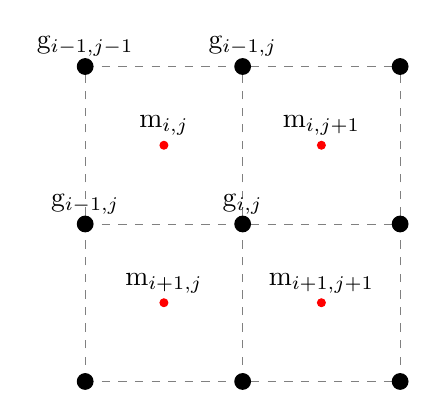
\begin{tikzpicture}

    \draw[style=help lines,dashed] (-0.001,-0.001) grid[step=2cm] (4,4);
          % Draws a grid in the new coordinates.
          %\filldraw[fill=gray, fill opacity=0.3, draw=black] (0,0) rectangle (2,2);
              % Puts the shaded rectangle
    \foreach \x in {0,...,2}{% Two indices running over each
      \foreach \y in {0,...,2}{% node on the grid we have drawn 
        \node[draw,circle,inner sep=2pt,fill] at (2*\x,2*\y) {};
            % Places a dot at those points
      }
    }

		\node[draw,red,circle,inner sep=1pt,fill] at (1,3) {};
		\node[above] at (1,3) {m$_{i,j}$};
		\node[draw,red,circle,inner sep=1pt,fill] at (3,3) {};
		\node[above] at (3,3) {m$_{i,j+1}$};
		\node[draw,red,circle,inner sep=1pt,fill] at (1,1) {};
		\node[above] at (1,1) {m$_{i+1,j}$};
		\node[draw,red,circle,inner sep=1pt,fill] at (3,1) {};
		\node[above] at (3,1) {m$_{i+1,j+1}$};

		\node[above] at (0,4) {g$_{i-1,j-1}$};
		\node[above] at (2,4) {g$_{i-1,j}$};
		\node[above] at (0,2) {g$_{i-1,j}$};
		\node[above] at (2,2) {g$_{i,j}$};


		\end{tikzpicture}


  \caption{lw}
  \label{lw}
\end{figure}

\item en esta implementación se calcula un solo array de puntos intermedios
\item en el primer paso se calcula u en los puntos intermedios $m_{i,j}$

\item para las variables ue, um (escalares):
\item $u_{m_{i,j}} = \frac{1}{4}  (u_{g_{i-1,j-1}} + u_{g_{i-1,j}} + u_{g_{i,j-1}} + u_{g_{i,j}}) - \frac{1}{4}\big[
\frac{dt}{dz_0} (f_{g_{i,j},0} - f_{g_{i-1,j},0} + f_{g_{i,j-1},0} - f_{g_{i-1,j-1},0} ) +
\frac{dt}{dz_1} (f_{g_{i,j},1} - f_{g_{i,j-1},1} + f_{g_{i-1,j},1} - f_{g_{i-1,j-1},1} )  \big] $
\item para la variables uc (vector) ():
\item $u_{m_{i,j},0} = \frac{1}{4}  (u_{g_{i-1,j-1},0} + u_{g_{i-1,j},0} + u_{g_{i,j-1},0} + u_{g_{i,j},0}) - \frac{1}{4}\big[
\frac{dt}{dz_0} (f_{g_{i,j},0} - f_{g_{i-1,j},0} + f_{g_{i,j-1},0} - f_{g_{i-1,j-1},0} ) +
\frac{dt}{dz_1} (f_{g_{i,j},1} - f_{g_{i,j-1},1} + f_{g_{i-1,j},1} - f_{g_{i-1,j-1},1} )  \big] $
\item $u_{m_{i,j},1} = \frac{1}{4}  (u_{g_{i-1,j-1},1} + u_{g_{i-1,j},1} + u_{g_{i,j-1},1} + u_{g_{i,j},1}) - \frac{1}{4}\big[
\frac{dt}{dz_0} (f_{g_{i,j},1} - f_{g_{i-1,j},1} + f_{g_{i,j-1},1} - f_{g_{i-1,j-1},1} ) +
\frac{dt}{dz_1} (f_{g_{i,j},2} - f_{g_{i,j-1},2} + f_{g_{i-1,j},2} - f_{g_{i-1,j-1},2} )  \big] $

\item leapfrog en el segundo paso: se calcula u en los puntos $g_{i,j}$
\item para las variables ue, um :
\item  $u_{g_{i,j}} = u_{g_{i,j}} - \frac{1}{2} dt  \big[ \frac{1}{dz_0} (f_{m_{i+1,j},0} - f_{m_{i,j},0} + 
f_{m_{i+1,j+1},0} - f_{m_{i,j+1},0} )  +  \frac{1}{dz_1}
(f_{m_{i,j+1},1} - f_{m_{i,j},1} + f_{m_{i+1,j+1},1} - f_{m_{i+1,j},1}) \big] $
\item para la variable uc:
\item  $u_{g_{i,j},0} = u_{g_{i,j},0} - \frac{1}{2} dt  \big[ \frac{1}{dz_0} (f_{m_{i+1,j},0} - f_{m_{i,j},0} + 
f_{m_{i+1,j+1},0} - f_{m_{i,j+1},0} )  +  \frac{1}{dz_1}
(f_{m_{i,j+1},1} - f_{m_{i,j},1} + f_{m_{i+1,j+1},1} - f_{m_{i+1,j},1}) \big] $
\item  $u_{g_{i,j},1} = u_{g_{i,j},1} - \frac{1}{2} dt  \big[ \frac{1}{dz_0} (f_{m_{i+1,j},1} - f_{m_{i,j},1} + 
f_{m_{i+1,j+1},1} - f_{m_{i,j+1},1} )  +  \frac{1}{dz_1}
(f_{m_{i,j+1},2} - f_{m_{i,j},2} + f_{m_{i+1,j+1},2} - f_{m_{i+1,j},2}) \big] $


\newpage





\item Lax Wendroff 2

\begin{figure}[ht]
  \centering
		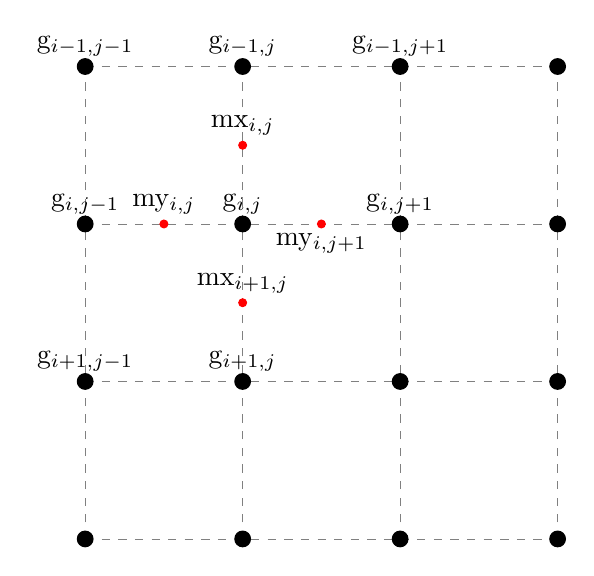
\begin{tikzpicture}


    \draw[style=help lines,dashed] (-0.001,-0.001) grid[step=2cm] (6,6);
          % Draws a grid in the new coordinates.
          %\filldraw[fill=gray, fill opacity=0.3, draw=black] (0,0) rectangle (2,2);
              % Puts the shaded rectangle
    \foreach \x in {0,...,3}{% Two indices running over each
      \foreach \y in {0,...,3}{% node on the grid we have drawn 
        \node[draw,circle,inner sep=2pt,fill] at (2*\x,2*\y) {};
            % Places a dot at those points
      }
    }

		\node[draw,red,circle,inner sep=1pt,fill] at (2,5) {};
		\node[above] at (2,5) {mx$_{i,j}$};
		\node[draw,red,circle,inner sep=1pt,fill] at (1,4) {};
		\node[above] at (1,4) {my$_{i,j}$};
		\node[draw,red,circle,inner sep=1pt,fill] at (2,3) {};
		\node[above] at (2,3) {mx$_{i+1,j}$};
		\node[draw,red,circle,inner sep=1pt,fill] at (3,4) {};
		\node[below] at (3,4) {my$_{i,j+1}$};

		\node[above] at (2,4) {g$_{i,j}$};
		\node[above] at (2,6) {g$_{i-1,j}$};
		\node[above] at (2,2) {g$_{i+1,j}$};
		\node[above] at (0,4) {g$_{i,j-1}$};
		\node[above] at (0,6) {g$_{i-1,j-1}$};
		\node[above] at (0,2) {g$_{i+1,j-1}$};
		\node[above] at (4,4) {g$_{i,j+1}$};
		\node[above] at (4,6) {g$_{i-1,j+1}$};
		\end{tikzpicture}


  \caption{lw2}
  \label{lw2}
\end{figure}

\item para las variables ue, um (escalares):
\item en el primer paso se calcula u en 2 arrays de  puntos intermedios $mx_{i,j}$ y $my_{i,j}$

\item $u_{mx_{i,j}} = \frac{1}{2}  (u_{g_{i-1,j}} + u_{g_{i,j}} ) - \big[
\frac{1}{8}\frac{dt}{dz_1} (f_{g_{i,j+1},1} - f_{g_{i,j-1},1} + f_{g_{i-1,j+1},1} - f_{g_{i-1,j-1},1} ) +
\frac{1}{2}\frac{dt}{dz_0} ( f_{g_{i,j},0} - f_{g_{i-1,j},0}  ) \big]  $

\item $u_{my_{i,j}} = \frac{1}{2}  (u_{g_{i,j-1}} + u_{g_{i,j}} ) - \big[
\frac{1}{8}\frac{dt}{dz_0} (f_{g_{i+1,j},0} - f_{g_{i-1,j},0} + f_{g_{i+1,j-1},0} - f_{g_{i-1,j-1},0} ) +
\frac{1}{2}\frac{dt}{dz_1} ( f_{g_{i,j},1} - f_{g_{i,j-1},1}  ) \big]  $
\item en el segundo paso:


\item $u_{g_{i,j}} =  u_{g_{i,j}} - \big[
   \frac{dt}{dz_0}  (f_{mx_{i+1,j},0} - f_{mx_{i,j},0} )+ 
   \frac{dt}{dz_1}  (f_{my_{i,j+1},1} - f_{my_{i,j},1} ) 
\big]$ 

\item de forma similar se calcula para uc


\end{description}



\section{Práctica}
\begin{description}
\item Definimos una amplitud A(en soundwave\_perturbation\_params.py) muy pequeña y una función periodica h en el intervalo $[x0_0, xf_0] x [x0_1, xf_1]$ (estos están en constants.py) con amplitud máxima 1 y creeamos las perturbaciones para que cumplan las relaciones entre las amplitudes de arriba y considerando una onda que empieza a propagarse en la dirección definida por la recta $n_x x - n_y y = 0$
\item definimos $ k_0 = \frac{n_x}{xf_0 - x0_0}, k_1 =  \frac{n_y}{xf_1 - x0_1}$ 
\item  $p\prime(x,0) = A \gamma p_0 h(x) $ 
\item  $\rho\prime(x,0) = A \rho_0 h(x) $
\item  $v(x, 0) =  A c_s h(x) (\frac{k_0}{|k|} , \frac{k_1}{|k|}) $ donde $|k| = \sqrt{k_0^2 + k_1^2} $
\item para el paquete de ondas (para el caso de propagación diagonal):
\begin{center}
\item $h(x) = e^{- \frac{(x_0-xc_0)^2 + (x_1 - xc_1)^2 }{W^2}} cos\big[2 \pi  K_0 (k_0(x_0 - x0_0) +  k_1(x_1 - x0_1)) \big] $
\end{center}
\end{description}

\paragraph{Fourier}

\begin{description}
\item para el caso 1d $h(x) = e^{-\frac{(x-x_0)^2}{W^2} } cos(k_0(x-x_0)) $ 

\item calculo con mathematica (de forma analítica) la transformada fourier de h con FourierTransform sin especificar FourierParameters que por defecto son  $0, 1$  y obtengo $f_3(k)$. De la documentación de mathematica y también se puede comprobar de forma analítica y numérica $f_3(k) = \sqrt{\frac{1}{2 \pi}} \int_{- \infty}^{\infty}{h(x) e^{i k x}} $ 
\item después de hacer unos cálculos:
\item $f_3(k) = \frac{W}{2 \sqrt{2}}  e^{-i  k  x_c}  (u_1(k) + u_2(k)) $
\item $u_1(k) = e^{-\frac{W^2}{4}  (k+k_0)^2} e^{-i  k_0 (x_0-x_c)} $ 
\item $u_2(k) = e^{-\frac{W^2}{4}  (k-k_0)^2} e^{i  k_0 (x_0-x_c)} $ 

\item \textbf{quiero representar de forma analítica y numeríca} $f_3(k)$
\item \textbf{de forma numérica}: calculo en python con scipy.fft $cp_n$, luego los valores $cp_n \frac{x_f - x_0}{\sqrt{2 \pi}}$  
y  $k_n = \frac{n}{x_f - x_0}, n = -N/2..N/2$ (el array se obtiene con fftfreq(N,dz))
\item \textbf{de forma analítica}: calculo de forma analítica en mathematica $f_3(k)$ (calculando la integral de forma explícita o con FourierTransform y calculo, luego calculo los valores $f_3(-2 \pi k_n)$ 
\item los represento frente a ($2 \pi k_n$)
\end{description}


\paragraph{Condiciones de contorno: reflexión}

\begin{description}
\item cambiando el parametro periodicType in soundwave\_boundary\_conditions.py  podemos  elegir las condiciones de contorno ("refl" o "repeat")
\item
\begin{figure}[!ht]
 \centering
 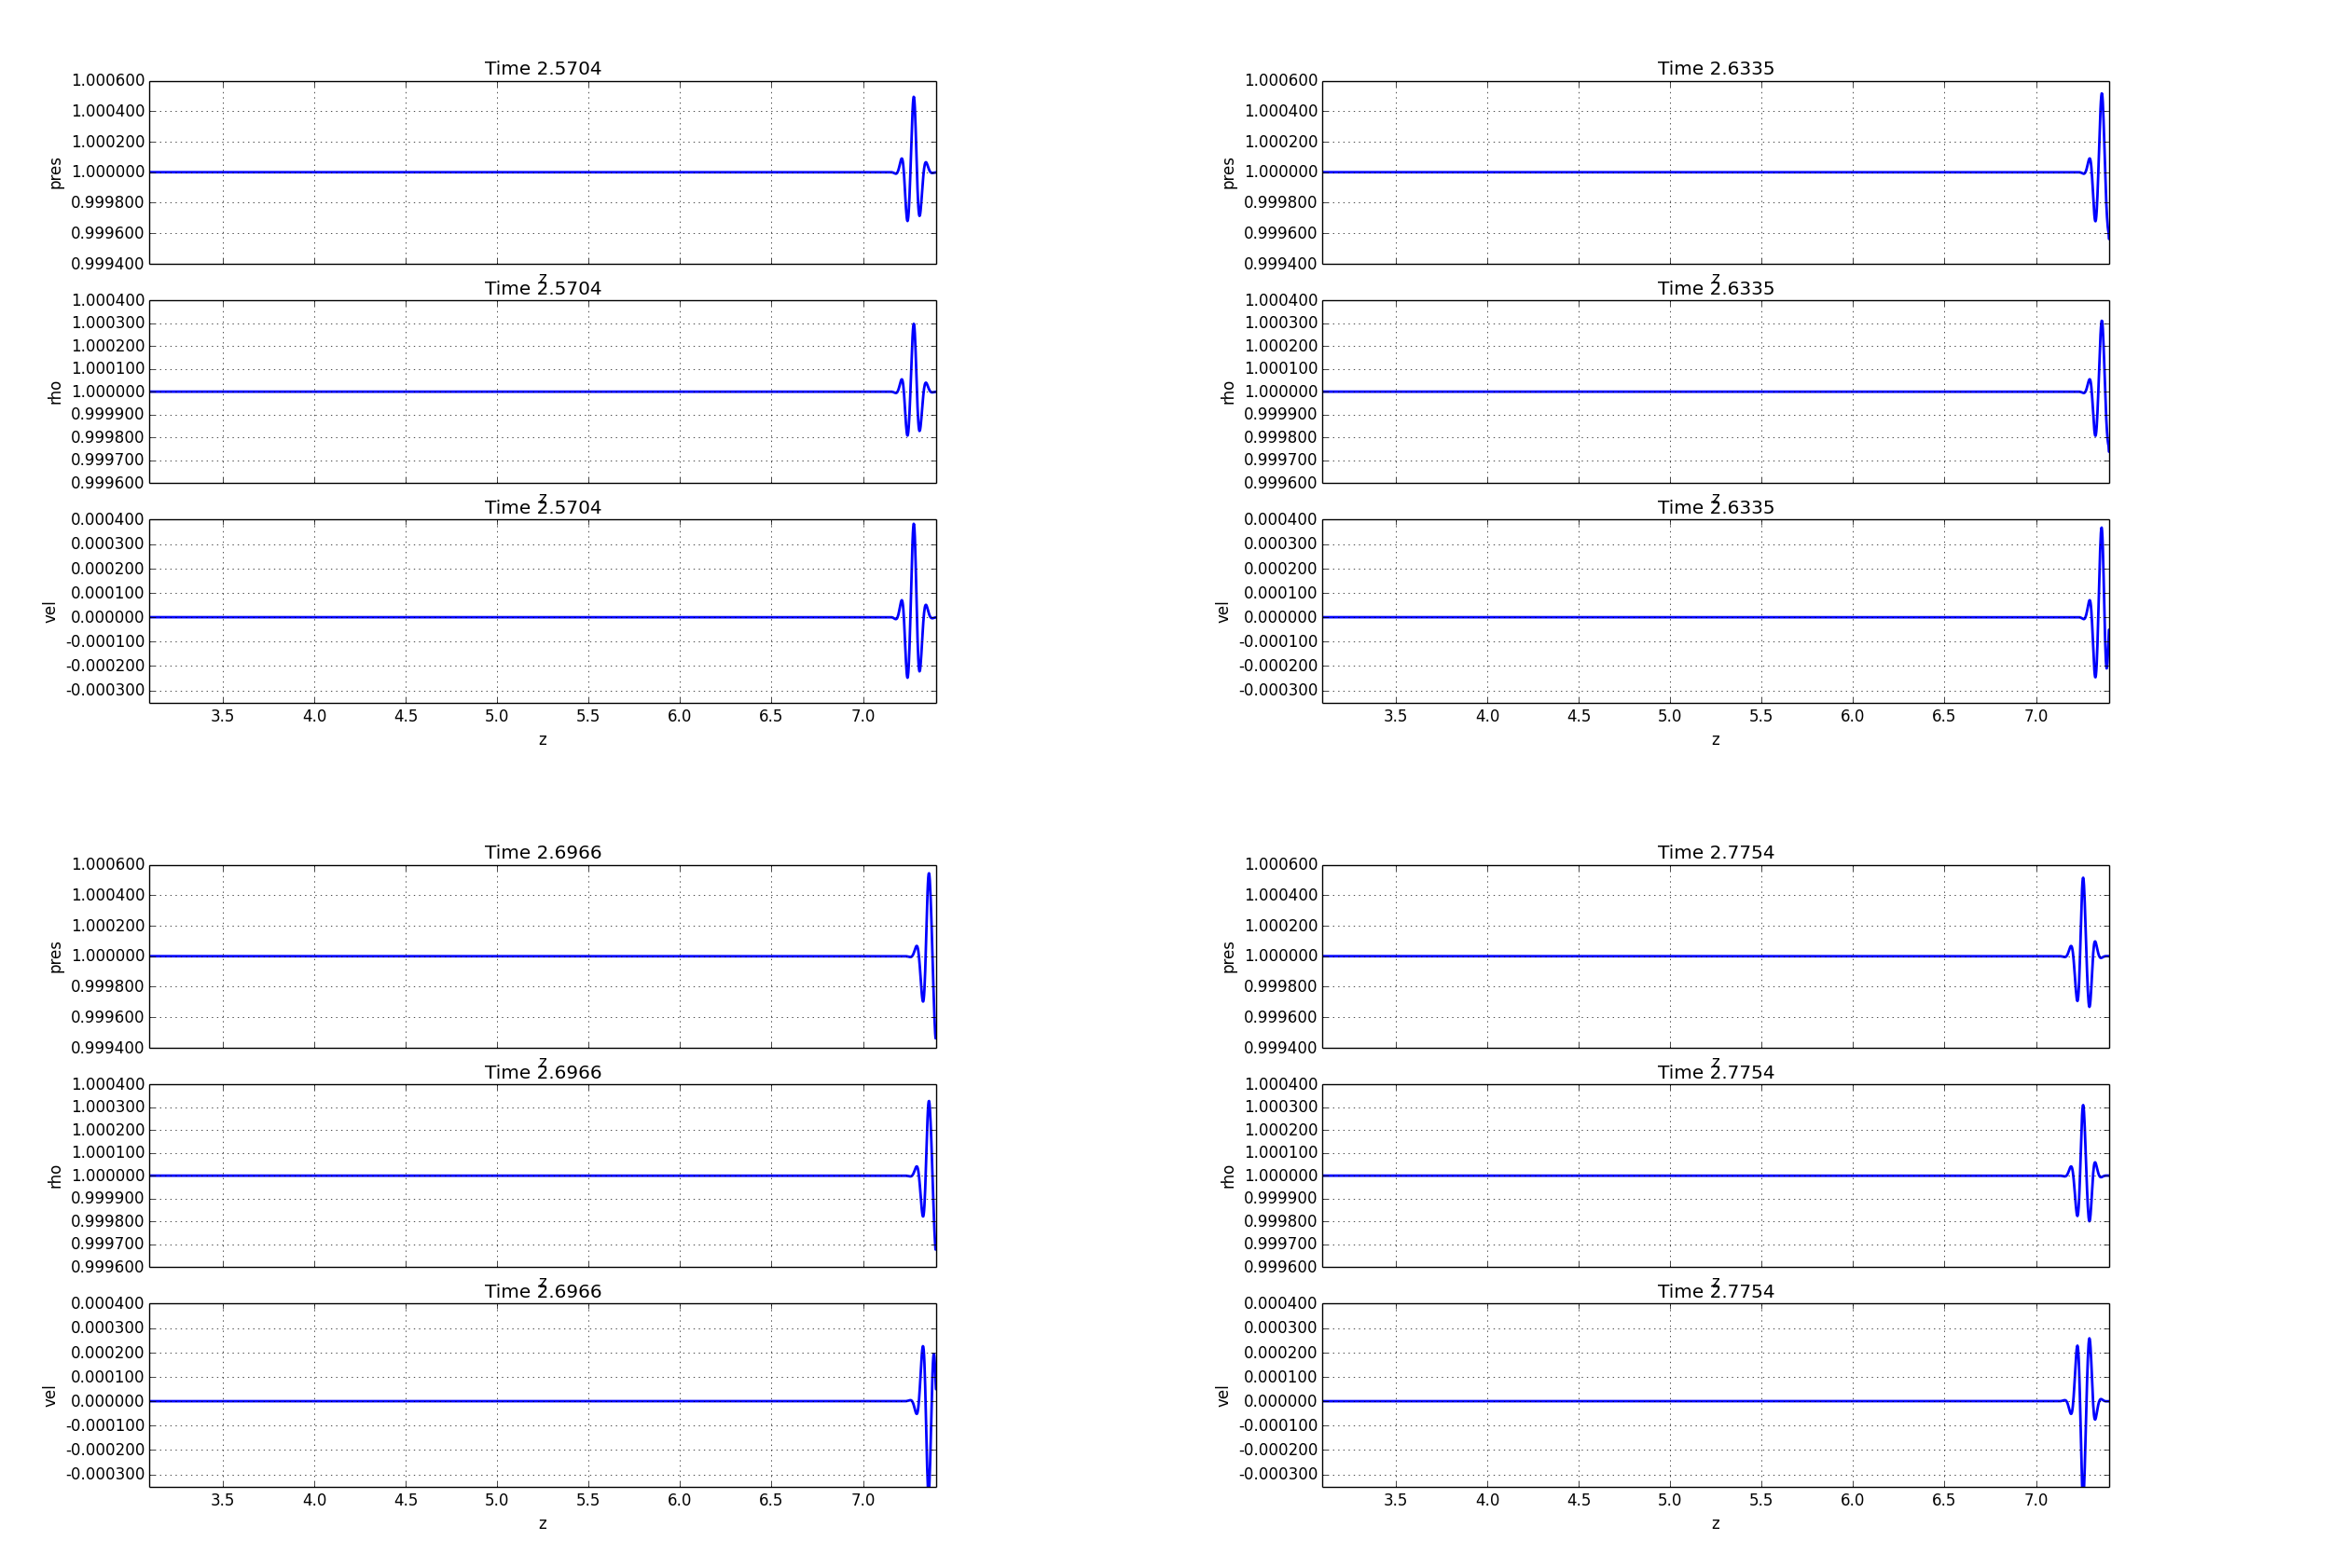
\includegraphics[scale=0.2]{reflhom.png}
 \caption{\emph{Evolución en el tiempo de las variables boundary conditions: refl }}
\end{figure}
\item TODO: la solución analítica con periodicType="refl" no está todavía implementada
\end{description}

\subsection{Medio inhomogéneo}
$p_0 $ const y $\rho_0(x) definida:$
\begin{center}
	$\rho_{00} + \frac{\rho_{01}-\rho{00}}{2}\big[ 1 + tanh(\frac{z-z_e}{w_e})\big] $
\end{center}

({\small las configuraciones del medio estan en soundwave\_medium\_params.py mediumType = "homog" o "inhomog" , $rho_{00}$ y 
los demás parámetros del caso inhomogéneo: $z_e, w_e, \rho_{01}$ })

\newpage
\paragraph{$\rho_0$ decrece }($\rho_{00} > \rho_{01} $)




\begin{description}

\item Evolución de la presión, densidad, velocidad, $rhoCurve = \frac{\rho- \rho_0}{\rho_0} $)

\item Las amplitudes de las perturbaciones de presión , densidad y velocidad  no son mas constantes al largo de los rayos como en el caso homogeneo igual que se ve en el gráfico de arriba, la amplitud de la presion y rhoCurve decrece y la de la velocidad crece (las time derivative  no son mas 0 como en el caso homogeneo)
\item En el caso homogeneo la solución para $\frac{1}{c_s^{2}} \frac{\partial^{2} h_2}{\partial t^{2}} = \frac{ \partial^{2} h_2}{\partial x^2}   $ con $c_s$ constante  y condición inicial $h_2(x,0) = h(x)$ en terminos de rayos se puede escribir:

\begin{description}
\item al largo del rayo $x_p(t)$ (solución de $\frac{dx}{dt} = c_s, x_p(0) = x_p$) 
\item $\frac{dh_2}{dt} = 0$ (time derivative)
\item equivalente a $h_2(x_p(t), t) = const = h(x_p)$  

\end{description}

\item De la ecuación de estado del gas perfecto: $T_0 = \frac{p_0} {\rho_0} \frac{\mu}{R}$, donde $\mu$ es masa molecular y R la constante de los gases
\end{description}

\newpage

\paragraph{Ray tracing}

\begin{description}
\item Marcamos en el los gráficos un punto $x_p = x_c$(el centro del paquete) y miramos la evolución en el tiempo desplazandolo en cada paso de tiepo con $c_s dt$. el punto se queda en el centro del paquete. Eso esperabamos porque los rayos son soluciones 
$x_p(t)$ de $\frac{dx}{dt} = c_g, x_p(0) = x_p$ y las amplitudes de las perturbaciones de presion, densidad y velocidad varian lentamente al largo de ellos  
\item en 1D $c_s=c_g$
\item la ecuacion de la variación de las amplitudes al largo de los rayos es válida para cualquier $x_p$

\item Sabemos de la teoria que al largo del rayo $x_p(t)$:
\item $k(x_p(t),t)  c_s(x_p(t)) = const$ 
\item Comprobamos la solución numérica: 
\item miramos la evolución en el tiempo de $k_c * c_s(x_p(t)) $ que debería ser constante = $k_0 c_s(x_p)$ 
\item  $k_c$ es el k para cual el valor de los coeficientes fourier $c(k)$ calculados con python 
de forma numerica con scipy.fft para el valor de la presión en el momento t es máximo 
\item pero tiene algunas variaciones como se ve en el gráfico:




\item $k_c$ no tiene orque ser igual al $k(x_p(t))$ ero si el paquete es bastante estrecho se considera que todos los k estan alrededor de $k_c$  y no pueden variar mucho. Para que esta condición se cumpla $\lambda << varLength$ donde 
$varLength =  min_{x}\big(|\frac{\rho_0}{\nabla \rho_0}|\big)(x) $
y $\lambda$ (wavelength of modulated wave) = widthPacket
\item la condicion $widthPacket < varLength$ se cumple solo al principio cuando el paquete era más estrecho


\newpage


 


\item En este caso como se ve en gráfico de arriba width(packet) crece y width(fourier) decrece.
\item La forma gauss del paquete inicial varia muy lentamente(el paquete sigue teniendo una forma (envelope) casi una función gauss se alarga un poco a la derecha si 
la densidad $\rho_0$ decrece y se estrecha  cuando $\rho_0$ crece) 
pero con W más grande y $f_1(k)$ una gauss con w mas pequeño cuando $\rho_0$ decrece y al reves cuando crece
\item De la expresión de la transformación fourier 
esperabamos tener una relación de proporcionalidad inversa entre width(packet) y width(fourier)
\item para no usar funciones que calculan de forma empirica la anchura del paquete  y de  $f_1(k)$ 
\begin{description}
\item determino la anchura del paquete siguiendo la evolución de 2 puntos (para la presión) que al principio están el el borde izquierdo y derecho (los meto con keys "left", "right"  en addMarkPoints en model\_soundwave.py, pero estos puntos los determino de forma empírica : los defino como $z_c$ - W*1.6,  $z_c$ + W * 1.6, W siendo el parámetro de la funcion gauss - definido en sound\_wave\_packet\_params.py) 
\item se que la anchura y el valor maximo de una función gauss son proporcionales 
\item mirando la evolución de $max(f_1(k))/widthFunction$ donde widthFunction es la anchura del paquete
no parece tan constante(hay que tener en cuenta la evolución lenta de la función gauss  que describe la forma del paquete? el periodo de tiempo representado es cuando el paquete pasa por la zona donde la variación de la densidad es mayor y la función se aproxima menos a la gauss):

\end{description}




\end{description}

\paragraph{Amplitudes}
\begin{description}
\item De las relaciones de  la evolucion teoretica de las amplitudes: en el caso cuando $ p_0$ constante $\implies$  
\item $|P(x_p(t),t)| c_s^{\frac{1}{2}}(x_p(t),t) = constant $ al largo del rayo $x_p(t)$
\item y las otras 2 se calculan de las relaciones : $\frac{|P|}{|V|} = c_s \rho_0 , \frac{|P|}{|V|} = c_s^2$
\item Las amplitudes se calculan al largo del rayo  $x_p(t)$ (la curva solución para  $\frac{dx}{dt} = c_s, x(0) = x_p$): $C_P$ es una constante que depende de los valores en el punto inicial del rayo ($x_p$): $C_P = c_s^{-\frac{1}{2}}(x_p) \rho_0^{\frac{1}{2}}(x_p)$

\item En la práctica he calculado la solución analítica de $|P|$ al largo del rayo $x_p(t)$:
\item $|P(x_p(t),t)| = c_s^{-\frac{1}{2}}(x_p(t)) c_s^{\frac{1}{2}}(x_p) P(x_p,0)  $
\item Para ver de forma empirica si paquete se adapta  a las curvas de forma  $const * cs^{\alpha} $representamos las curvas:
\item para la presión: $ c_s^{-\frac{1}{2}}(x) c_s^{\frac{1}{2}}(x_0) P(x_0,0) $
\item densidad: $ c_s^{-\frac{3}{2}}(x) c_s^{\frac{3}{2}}(x_0) R(x_0,0)  $ 
\item velocidad: $ c_s^{\frac{1}{2}}(x) c_s^{-\frac{1}{2}}(x_0) V(x_0,0)  $ 
\item eligiendo $x_0$ los 2 puntos donde  los valores de las amplitudes de las perturbación en el momento inicial tienen el mínimo y máximo 
\item ya sabia que $\alpha = -\frac{1}{2}$ para la presión, $\alpha = -\frac{3}{2}$ (para la densidad, $-\frac{1}{2}$ para rhoCurve), $\alpha = \frac{1}{2}$ para la velocidad (pero se puede variar tambien en el grafico: ver model\_soundwave.py)
\end{description}

\textbf{Conclusiones}:
\begin{description}
\item Por la forma que tienen las ecuaciones diferenciales de las variables de cuales queremos estudiar la evolución:
\item $\frac{\partial p}{\partial t} + c_s \frac{\partial f}{\partial x} = g(x,t)$
\item la solución se puede expresar usando el termino de rayo(creo que se llama de otra forma?)
\item definimos el rayo $x_p(t)$ la solución de la ecuación $\frac{dx}{dt} = cs, x_p(0) = x_p$
\item la PDE de arriba se transforma en DE al largo del rayo $x_p(t)$:
\item $\frac{dp}{dt} = g(x_p(t), t)$
\item $k,\omega, \phi, E, a$ tienen relaciones que se pueden expresar como diferenciales de tiempo al largo de los rayos. 
\item la dependencia de x se transforma en dendencia de tiempo y de $x_p$ el punto inicial del rayo (al momento t=0)
\item $\frac{d\phi}{dt} = 0 \implies $ el paquete no cambia de forma pero su anchura crece(k decrece) cuando $ c_s$ crece y se estrecha cuando $c_s$ 
decrece de forma proporcional a k (por la relación: $\frac{dk}{dt} = -k \frac{dc_s}{dx}$)
\item de la ecuacion diferencial de  la amplitud al largo del rayo (o de la energía) se obtiene una relación genérica de dependencia de la amplitud  de $c_s$ , $\rho_0$ , $p_0$ que tiene  que cumplir las 3 variables : perturbacion de densidad, presión, velocidad
\item pero de la ecuación de movimiento de los fluidos y de la condicón de adiabaticidad se obtienen otras 2 relaciones entre las amplitudes de cada una
\end{description}

\newpage 


\newpage 
\subsection{Documenatción usada}
\begin{description}
\item \href{http://www.awi.de/fileadmin/user\_upload/Research/Research\_Divisions/Climate\_Sciences/Projekt/1\_to\_3\_\_WO\_waves.pdf}{http://www.awi.de/fileadmin/user\_upload/Research/Research\_Divisions/Climate\_Sciences/Projekt/1\_to\_3\_\_WO\_waves.pdf}
\item \href{https://classes.soe.ucsc.edu/ams227/Fall13/lecturenotes/Chapter2-part2.pdf}{https://classes.soe.ucsc.edu/ams227/Fall13/lecturenotes/Chapter2-part2.pdf}
\end{description}
\subsection{Codigo}
\begin{description}
\item  Todo el código está en el repositorio git:

\href{https://github.com/beevageeva/simnum/}{https://github.com/beevageeva/simnum/}

en la carpeta D1-python
\item Si no quiere usar git también hay un archivo comprimido de los ficheros *.py en:
\href{https://github.com/beevageeva/simnum/blob/master/D1-python.tar.gz}{https://github.com/beevageeva/simnum/blob/master/D1-python.tar.gz}

\item Para ejecutar (timeEnd por defecto = timeEnd definido en constants.py):
\begin{verbatim}
	python main.py --timeEnd=5
\end{verbatim}

\item Los parametros de configuración están en:
\begin{description}
\item soundwave\_boundary\_conditions.py 
\begin{description}
	\item periodicType = "repeat" | "refl"
\end{description}

\item soundwave\_medium\_params.py los parámetros relacionados con el medio : mediumType("homog" o "inhomog") ,$p_{00}$, $v_{00}$, $rho_{00}$ y  en el caso del medio inomogeneo: la funcion de densidad inicial
\item soundwave\_perturbation\_params.py los parámetros relacionados a las condiciones iniciales (la perturbación): el tipo de la función y para cada tipo definido aqui hay un fichero distinto donde se configuran los parámetros de cada uno: en el caso del wave packet este fichero es sound\_wave\_packet\_params.py , la amplitud. También se pueden definir superposisiones de funciones. 
\item constants.py: 
\begin{description}
\item  gamma = 5.0/3, z0, zf, nint,timeEnd, schemeType = "lf" (lax-fr) | "fg" (first generation), fcfl, loopType="python" | "weave"
\item loopType = "weave" $\implies$ los calculos de las derivadas en alg.py se hacen en C. Tambien para calcular la solución analítica en
analytic\_solution.py 
\item en el caso de schemeType="fg" se especifica el paso cuando se aplican las condiciones de contorno: en el paso final bcStep = "final" o en el paso intermedio bcStep = "interm"
\end{description}
\item en notifier\_params.py están los parametros relcionados con los gráficos: nStepsPlot = 10 (solo repinta los gráficos cada 10 iteraciones)
y si pintar algunos gráficos o no como por ejemplo rhoCurve o fft fourier o fft fourier sol analítica o la sokución analítica
\item la solución analítica no está implementada para cond contorno reflexión
\item hay mas parámetros que se pueden cambiar que estan la principio de los ficheros python: en visual\_plot.py donde están las funciones relacionadas con los gráficos se definen los xlim, ylim, saveImages = True (guarda una imagen en la carpeta outImages\_*) y en model\_soundwave.py como addMarkPoints que es un hash de los puntos de cuales queremos ver la evolución (en cada iteración los dezplazamos con $c_{s}$ * dt) $c_s$ calculado numérico de los valores de la presión y densidad (funciona con superposiciones) . 
\item Para calcular la anchura del paquete hay que añadir a addMarkPoints los puntos que inicial están a los bordes del paquete con los keys: "left"  y "right" porque la anchura la calculo siguiendo estos 2 puntos (mejor que con funciones que determinan la anchura de forma empirica: determinando los z cuando la funcion  empieza a ser diferente de la derecha y izquierda)
  

\end{description}
\end{description}
\end{document}


